\section{Chatbot performance}
The nature of chatbot development is one of predicting what a user will say; this is already a hard job for any large software development effort, making it incredibly difficult for a single person team.
Testing on our own account, using phrasings we knew the chatbot would recognise, was very different from deploying it in the wild, and experiencing all the different ways participants in the study tried to express the same concepts.

Observing how the users were interacting with the chatbot made it clear that our design choice of minimising false negatives by using the \textit{@sys.any} entity to capture food was not particularly successful. Users would often try to interact with the chatbot for non functional conversation, such as greeting it, thanking it about one of its encouragements to keep logging food, complaining about a mistake or simply acknowledging a previous message. In those cases, if the intent-triggered conversation had already been terminated, the new message would be incorrectly identified as food, without a quantity, and a clarification request message to specify the portion size would be fired. \\
\begin{figure}[h!]
  \centering
  \begin{subfigure}[b]{\linewidth}
    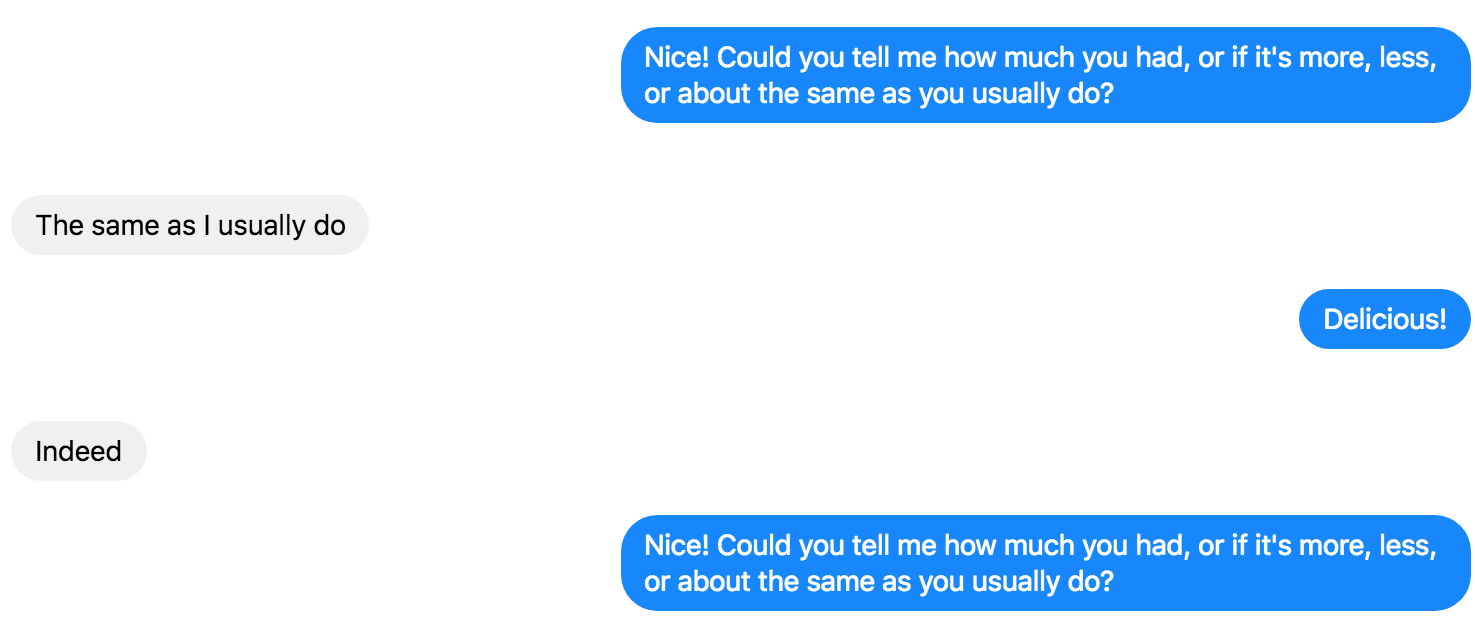
\includegraphics[width=\linewidth, height=6cm,keepaspectratio]{Nice.png}
     %\caption{Coffee.}
  \end{subfigure}
  \begin{subfigure}[b]{\linewidth}
    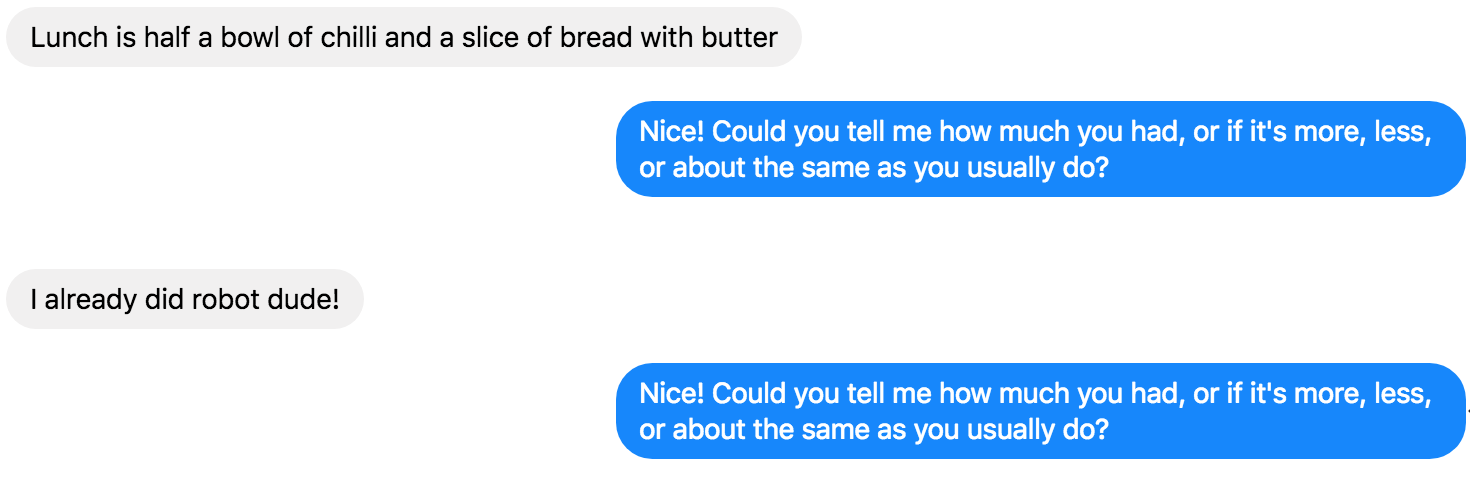
\includegraphics[width=\linewidth, height=6cm,keepaspectratio]{Nice2.png}
    %\caption{More coffee.}
  \end{subfigure}
\end{figure}
This also caused the intent recognition model to have several false positives, misidentifying stop words as food within a message that also contained valid food words. Fortunately, this kind of errors turned out to be less relevant, because the user would already have to identify some portion sizes, so they would not notice misidentification issues, and the recognised food was only stored in the database if matching with some record in the \textit{Nutritionix} API. \\
But while the API did provide a safeguard against incorrect food identification, it also showed issues by misidentifying real food, either by catching only part of the word (cupcake was flagged as cake mix in one instance), or sometime inexplicably (Long island ice teas were stored in the database more than once, without the user having logged them). The ability to list several different food items within a single message, as well as users' habit of splitting up different elements of the same meal between different messages, also caused difficulties in matching quantity to food, with Dialogflow's models simply not being advanced enough to catch the many subtleties of word ordering. This was another cause for the size clarification message to be presented after a quantity had already been given.

The \textit{clarifai} API rarely conformed to our ideal parameter of a single identification over the 97\% confidence threshold; however, the among the top three choices, there was often a good candidate the user could choose to select. When confronted with no suitable choice, if the user tried to clarify what the food was, the chatbot appeared to recover gracefully, while actually logging the clarification as a new meal. 

A considerable effect on how the chatbot performed with users was also due to operational issues. After obtaining consent to participate in the experiment, users were provided with a URL they could open through the Facebook Messenger app or in the browser. Before it became clear that individual users had to be added as testers through the Facebook developer console, the first users who were given a URL did not receive any reply to their messages until they were added. While it was explained to them that this was not an issue with the chatbot but a temporary account management problem, it might have contributed to the perception that the chatbot was buggy. In fact, even after testing initiated correctly, there were some uncaught bugs that users could easily spot, which betray the fact that they were conversing with an automaton. For many of the chatbots' interactions, responses were selected randomly from a predefined list; over time, the user would exhaust all variants for a response, and since these were selected randomly sometimes would have the exact same responses given to them in quick succession. Sometimes, the database would fail silently when accessing the user name, so a message would be sent to the user containing ``undefined'' rather than their name. \\
Perhaps most grievously, an uncaught exception in the logic of \textit{worker.js} caused the entire periodic reminder script to fail after having sent messages to the first user. Because the first user was our test account, we kept receiving reminders through the evaluation period, which caused us to believe everything was behaving correctly until the 6th day of the experiment. Since this was a very important feature we were interested in evaluating, we decided to push a fix in production, and to extend the trial by two more days to verify its effects. We deactivated the reminder for feedback after 3 days had passed, because with the change in schedule it would have fallen too close to the conclusion. \\
The fix was not perfect, causing the no log reminder to fire up for every user, even if they had just logged their food the night before. However, while this might have been annoying for these users, it proved highly effective, causing every single user to log at least a meal on the day and after, including those who had only tested it on the first day and given up after. The leafy greens reminder was also subjected to a similar bug, firing for every user just before the no log reminder. Unlike the latter, most users did not seem to react to the suggestion, and while some registered the message, it is unclear whether users failed to modify their behaviours because the greens reminder encourages a more difficult change, or simply because they only noticed one of the remainders. The second explanation is not unlikely, given the fact that our testers seem to ignore larger body of text while messaging, like the introductory welcome message which explained the chatbot's capabilities, causing users who were not given an explanation before the experiment to be unaware of some functionality. 

Another functionality that was not presented to the user due to some small logic errors was the undereating reports. One of the condition for undereating was that if only two small items of food were inserted before 11 PM, we should flag an undereating option; this however should only have applied if the request was made for food on the current day, causing previous days' requests executed before 11 not to trigger. This issue might however be considered negligible for the purposes of our evaluation, since users rarely asked for previous days' logs, and those that did never fulfilled our conditions to trigger an overeating message.
\section{Evaluation results}
While our study provides us with some interesting qualitative data, it should be noted that we cannot conduct hard generalisations on our results, because of the tiny sample size. Our participants come from the uniform demographic of university students because of issues with the logistics of recruitment; while this enables us to compare data without taking into account how demographics affect replies, it also means we lack external validity, and we cannot understand how other groups, especially in vulnerable less tech-savy age groups or with have major dietary issues, will react. Further studies will be necessary to ascertain how usable the interface is for different demographics. 

Responses to our survey confirmed that the chatbot is not ready for public release, and in its current incarnation provides little utility compared to app based food diaries; however, under some metrics the chatbot did provide a stronger performance, leaving open the possibility that with more work it might provide a suitable replacement. \\
More than one participant did note that interacting with the food log through conversation was, despite the frustrations with some faulty NLP, a benefit over MyFitnessPal, even wishing that the conversations could be more human like. In fact, while more users rated MyFitnessPal as being useful compared to the chatbot, the chatbot was rated as more pleasant to use than the app, despite the bugs. \\
Some evidence that the chatbot interface is easier to interact with than the MyFitnessPal menu can be glimpsed from the fact that a higher proportion of users did not log their meals because they were too busy or it would have been too much of a hassle. Indeed, there were complaints about the speed of entering a meal into the app being too slow.\\
Conversational interfaces also seem to influence users' thoughts on how food should be measured in logs, with participants who were exposed to chat marking a preference for keeping measurement relative to previous meals, as opposed to MyFitnessPal users preferring absolute measurement. This can be attributed as a reflection on the functionality provided by the two systems: our chatbot does not provide precise calorie counting calculations, making it less important to have a precise metric on how much food has been eaten. This can make food logging easier, because the user does not need to worry about using a scale or counting portions, but only need to give the easy estimation on how much they have eaten compared to previous meals. Of course, having precise quantity would enable us to perfect data analysis on the backend, but having a relative measurement already allows us to build simple heuristics such as ours to detect any new over or undereating trend in the users' habits, and there are some research projects looking into using machine learning to supplement missing health data \cite{wolters}. \\
Conversational reminder seem to be more effective than regular app notifications: every user of the chatbot logged a meal after receiving a reminder, while MyFitnessPal users who had turned on reminders did not act on them, or reported that they probably would not have been convinced by a reminder to log food. This of course might have been caused by the sparsity of reminders, since we never sent any in the first few days of the trial, and reminders to take actions outside the chatbot, like eating some leafy green vegetables, were not acted on. Nonetheless, users seemed to react favourably to the feature, and even requested having more frequent notifications to avoid skipping further meal logs. 

The most important outcome from the survey that we did not observe during the previous evaluation trial was the issue of feature discoverability. Our solution of simply stating the chatbot functionalities in the opening message did not work, causing a significant number of participants not to be aware of features like picture logging or past logs requests. Users also reported not knowing about the analytics function the chatbot had, but those were intentionally left vague in the welcoming dialogue. The onboarding information was presented as a rapid succession of messages, which were also longer than usual, and the combination might have proven too much for the users who just scanned their content quickly. We also provided a helper message in case someone needed reminders on how to use the bot, but it was never invoked. Potential solutions to this issue include improving the initial dialogue, making it more interactive, breaking down the onboarding into a more gradual set up over the first day, or, taking a page from what most current Facebook Messenger bots do, using a persistent menu, which somewhat nullifying the benefits of having a conversational interface, and always presenting all features as quick reply options at the end of a previous conversation. This approach is highly recommended, as it provides user with a visual list of all input possibilities, as well as giving the chatbot a good understanding of what the user is intending to do, effectively resolving issues such as our chatbot's tendency of misclassifying an excessive amount of messages as food insertions. While we had been aware of this approach during development, we chose not to use it because in our opinion it broke the suspension of disbelief of having a conversation with an intelligent agent; in retrospect, it would have greatly improved our design, and it would be easier for user than being explicitly \textit{trained} into using the correct formulation to match an intent. 

Across both platform, we saw a common trend of users not being able to draw any utility from the logging because they considered themselves to already have a good grasp of their diet. As much as users may believe that is the case, the advantages for more conscious users will emerge through further data analytics over larger period of times to identify long term trends, and better visualisation tools to display more useful information. In the case of the chatbot, since textual feedback is somewhat limited in the type of information we can display to the user, it would be beneficial to insert a webview within the Messenger app, which could enable us to display rich graphical content (the Forksy chatbot has a nice graphical overview for a user's food diary). \\
\begin{figure}[h!]
  \centering
  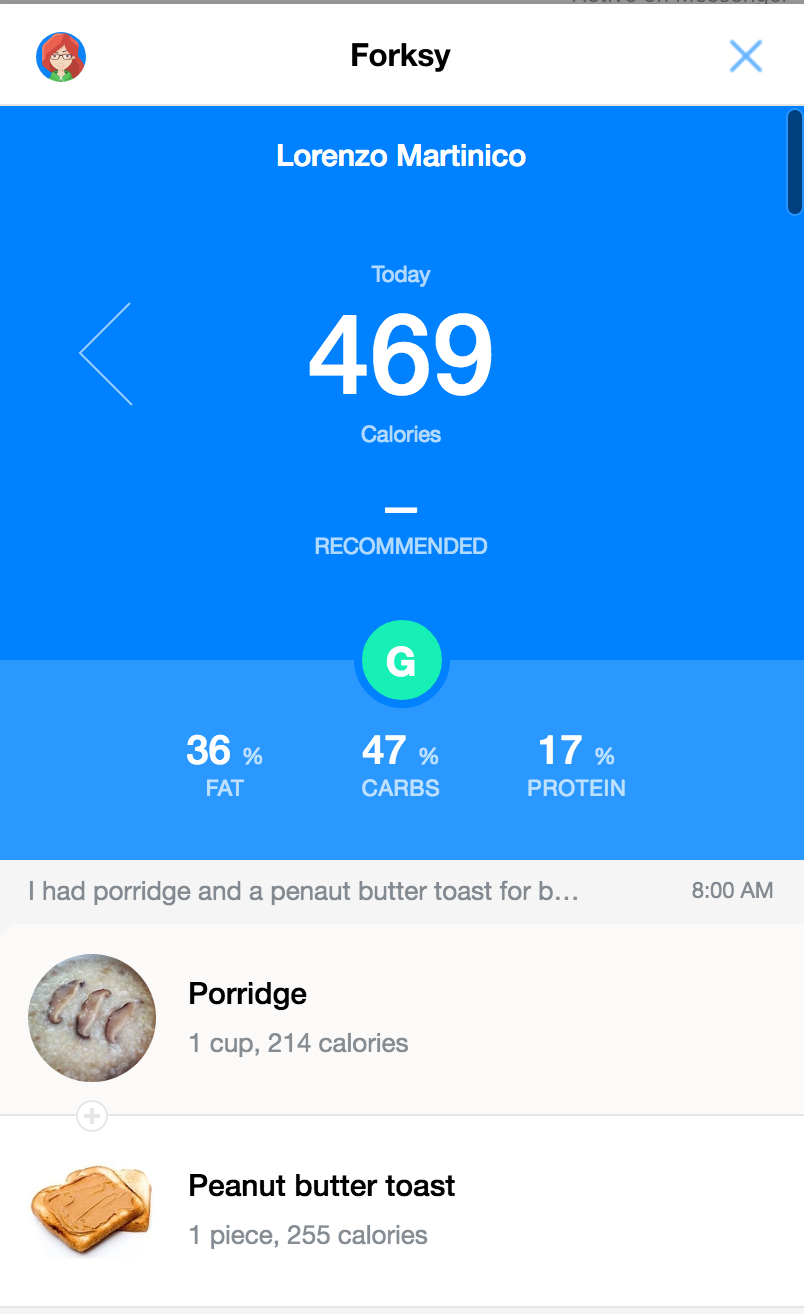
\includegraphics[height=14cm, keepaspectratio]{Forksydiary.png}
  \caption{The Forksy food diary}
\end{figure} 

More adequate feedback could also be provided by taking into account users' goals and dietary preferences. It is meaningless to send a warning for having too little or too much food if we do not know whether the user is trying to lose weight or training to build muscle, and it might be harmful for users who already struggle with dieting to receive feedback their not having enough nutrients. Knowing whether a user is on a special diet, such as vegetarian or vegan, would also be beneficial, both for keeping track that users are getting all their nutrients, and to avoid making inappropriate recommendations for food that is missing from their diet. 

Since our chatbot deals with people who may be in the vulnerable frame of mind of being insecure about their diet, we have to take extra care of what users are saying. Running some sentiment analysis on user input may avoid tragically inappropriate exchanges such as this, caused by the random selection of encouraging phrases in response to logging food, which besides making the user feel mocked also betrays our lack of understanding of the input's context. \\

\begin{figure}[h!]
  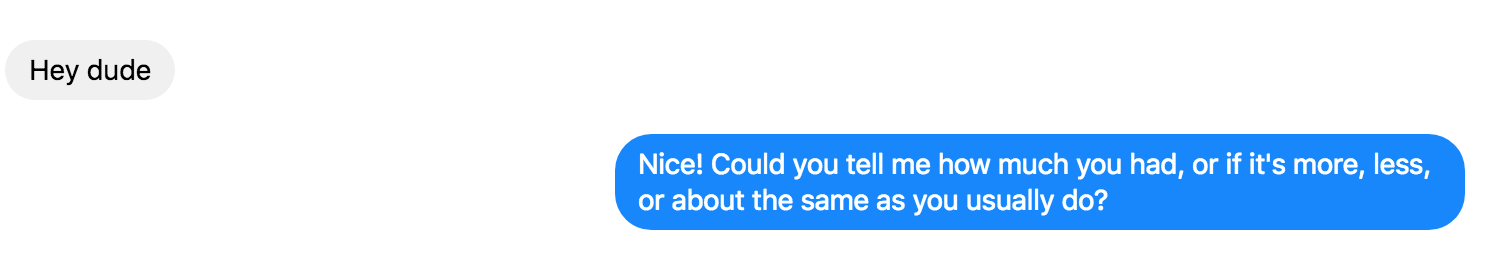
\includegraphics[width=\linewidth, keepaspectratio]{Nice6.png}
\end{figure}

Some interesting feedback we received through the surveys was about user's mental model of how the chatbot worked (or rather, didn't). Users attributed undue relevance to the ``seen'' message icon on the Messenger application. While this would appear whenever a reply was sent, it would remain unmarked when the chatbot received a message it did not acknowledge it. The lack of read receipt co-occurred in some occasions where some expected remarks were not sent, most likely due to the Heroku server not waking up in time, causing users to associate the two events. Similarly, after the erroneous reminder for lack of usage was sent overnight, participants reported the chatbot not being able to distinguish whether they were sleeping or putting off logging food. These assumptions can be powerful to leverage when designing our conversations, by exploiting users' misconceptions to cover up flaws in the dialogue system. More studies should be conducted in this area. 

\section{Future improvements} 
% maybe goes in conclusion?
There are many directions in which a project like this could go, and while our implementation was a bit barebones and only offered the essential features, there are several things we thought of during development or received requests from users which we might have added to make for a more useful and complete nutritional assistant, but had to hold off from because of time constraints. 

An immediate feature addition that was reported as being useful during evaluation, was the option of retroactively adding a meal to the previous day. We immediately added the feature, which was a simple fix of changing the date object in the MongoDB update code from statically being the current date to taking the intent's argument. We did not push the new feature however because we were concerned deploying it would affect current users. 

To match our functionality with MyFitnessPal's, we should also allow easy scanning of commercial food packages through a barcode scanner. While we could enable scanning on submitted images, this could lead to negative user experience when testing with badly framed images, requiring several photographs of the food to be taken before a match would be identified. Instead, we could rely on a Facebook Messenger webview object to integrate a live barcode scanner\footnote{possibly integrating https://github.com/serratus/quaggaJS}, but it is uncertain how well it would perform. 

People interact in different ways with modern messaging platforms, and our chatbot should be able to take advantage of these new forms of communications: emojis, stickers, gifs. There are tagsets to classify this rich content based on emotion expressed, so we could use this as a basic form of sentiment analysis for incoming message, and to express personality when sending outgoing messages. We already have some hardcoded emojis as part of our script, but adding stickers and gifs to a generative model for text would make the chatbot feel more like a real entity, since the number of options is very large compared to the number of scripted responses we can write. 

Some people tend to have a very regular diet, where they will eat the same meal for several days in a row. MyFitnessPal acknowledges this, and it provides an option to copy a meal from a previous day. This interaction pattern would fit naturally with a chatbot dialogue, where a user could simply say: ``I had the same breakfast as yesterday'', and the system should just replicate the same food as in the previous day. Of course, this would require enforcing a more strict separation between meals that we currently have, but we could guess it based on time of input, or by simply setting the meal type as a required parameter in the logging intent. Even simpler, although a bit less natural, would be asking the chatbot to set a recurring meal to be copied every day until manually interrupted. 

A feature that was particularly appreciated by MyFitnessPal testers was recipe suggestions. It would be good if the chatbot could automatically suggest recipes, based on what nutritional requirements the user needs to fulfil, and maybe taking into account dietary history and preferences. In fact, with enough food data it might be possible to infer what kind of foods the user likes, and aggregating data across several users we might be able to provide a recommender system for discovering new recipes you might not know. 

A nutritional assistant should also be able to give you some advice on specific food. It would be pretty simple to add an intent to query information from the \textit{Nutritionix} API about the nutritional values of the food in question. However, the challenging aspect of such a feature would be displaying the information in a useful way. It could be possible to display nutritional content in grams for each macro and important micronutrients, but that would only benefit people who can understand what those nutritional values mean, and does not fit within the final aims of our chatbot. Perhaps contextualisation with past meals might provide useful, but we need to be able to classify what kind of food that is, which is still an unknown problem.

We should also be interested in tracking other factors beside the food eaten. Sleep, mood, level of stress and exercise are all massive factors that can affect and be affected by what we eat \cite{buman2015physical}. The chatbot should capture these factors, either by interfacing with another quantified self platform, or by asking users questions at the start of the day. \\
The above features would mostly be relatively straightforward to implement, and we would have added them to our chatbot if we had had more development time available. We also envisioned several other possible features, which would be interesting, but would also require a lot more work to make possible.

An interesting component in diet tracking is social awareness, as discussed in the Background chapter. While the chatbot interface in itself does not provide any obvious advantage from this point of view, the network effect of having an agent that can interact with your contacts, be it your social circles in Facebook Messenger or your co-workers on Slack, can provide some interesting opportunities to leverage social pressure. The most immediate idea is having the chatbot set ``challenges'' to a group of users. This might take the form of a user invoking the chatbot in a group chat through the Facebook Chat Extensions \cite{chatextensions}, and setting a randomised ``healthy eating'' challenge (something along the lines of \textit{eat 5 portion of vegetables every day for the next week}). The chatbot would then end ask for participants among the group chat members, and once everyone has accepted or declined the challenge, it would keep a score of how everyone is doing, publicly complimenting those who are on track and encouraging who has been lagging off to do better. To avoid polluting the group chat, whose purpose might not be just having fitness challenges, logging should happen within the regular direct message interaction with the chatbot, and shoutouts and encouragements should be limited to a small daily window. \\
The idea of using the chatbot has a motivator tool to set challenges against themselves could also be expanded to the context of an individual user. This would work very similarly to the group challenges, except the user would be competing against themselves, trying to surpass their previous goals or stick with a new healthy habit. 

We would also like to go back to our original idea of integrating images from social networks. With Instagram being impossible to use (besides scraping public facing profiles through a crawler), Flickr seems like the best alternative. Syncing with a user's photo collection allows us not only to save time from logging their new meals, and to capture a snapshot of historic data, but also leverage metadata that the social network makes available to us, such as image tags and the social graph of people interested in that picture. This would help strengthen the prediction for our food classification, but would also provide a basis to group related foods together. 

Another helpful deception our chatbot could adapt, until an appropriate nutritional knowledge base and algorithms to understand an individual's diet can be developed, would be giving a trained nutritionist the possibility to examine data that has been submitted so far, and intervene to give appropriate advice. Facebook Messenger does expose a Handover protocol \cite{handoverfacebook}, designed for such a case where a human operator needs to takeover the chatbot's operations. We would also need to have some visualization tool, so that the human nutritionist might understand at a glance what the situation is and offer the necessary advice.
\section{Chatbots and privacy}
Throughout our implementation and evaluation phases, it became evident how little privacy a chatbot user can expect. Participants on our experiment, who come from a variety of academic background, mostly showed having some expectations of privacy, regardless how much they were concerned about the confidentiality of this specific domain, and overall customers across Europe report greater concerns with how their personal information is being handled by private companies \cite{europasurvey}. 

In our architecture, we had several stages where data was ``leaked'' to a third party: all communications between users and chatbot were completely accessible to Facebook, as the provider of the Messenger platform, and us, as well as any other potentially malicious administrators to the Facebook page the bot was linked to; all conversations were also forwarded to Google, to be analysed as part of their Dialogflow service; food eaten was stored on our MongoDB provider website; and some logs were leaked to the Heroku instance from our webhook code, which potentially could have stored a lot more information than it did. All of this data was associated with a personal identifier, or even the user's own name. \\
While ideally we should be able to trust these service providers with user information, revelations in the last few months have increased user's awareness, and concerns, with certain data brokerage and collection practices that are common among the tech giants, which leave data vulnerable to be exploited by malicious agents. And while the sensitivity of nutritional habits may not seem important, up until you consider how major eating disorders might be considered by insurance companies, using a chatbot in any other medical setting might be a cause of concern. Narrow rules in the United States govern how medical sensitive informations can be dealt with (regulated by the Health Insurance Portability and Accountability Act), and soon Europe will enforce data protection on its citizens (through the General Data Protection Regulation). 

While most of the major messaging platforms nowadays provide an option for end-to-end encryption, especially thanks to the Signal Messaging protocol \cite{signal}, which has been widely deployed through industry, no one provides facilities to encrypt chatbot conversations \cite{Alesanco2018}, except the Wire messaging app, which has a barebones chatbot API in alpha stage (but it is unclear whether it is actually being used beyond their initial demos \footnote{https://github.com/wireapp/wire}), and the Matrix protocol \footnote{https://github.com/matrix-org}, which allows chatbot users within encrypted channels, but does not provide an officially documented API to develop them, which means there are about a dozen customly developed bots available. \\
While an API such as Wire's uses end-to-end encryption to protect messages from the platform provider, a user still has to trust the other end, whoever controls the server the chatbot runs on, not to steal their data or leak it to malicious third parties. It might be possible to mitigate this risk with a revised client-only chatbot architecture, where some basic parsing happens immediately on the client side, perhaps using historic chatbot technologies such as AIML \cite{aiml}, or some ondevice machine learning, which has become more feasible in the past few years \cite{tensorflow}. This architecture would still include a server, whose only function would be storing the encrypted data, and conduct the relevant data analytics in an anonymous and confidential manner by using zero-knowledge proofs, an encryption scheme which enables a system to prove properties of a message without decrypting it. Of course, this would probably prevent more complex natural language processing which requires large scale data analysis, but maybe with proper conversation design it could be enough to maintain all important functionality, and any necessary data collection to improve on-device machine learning models might be conducted through privacy preserving techniques.
% cite MFP hack!!
% elaborate on dealyed interval's effectiveness